\chapter{Implementation}

The first stage of this research was to implement the motion imitation with ZMP balance control. This implementation helps the initial validation of the capabilities for real-time motion imitaion, 
as well as processing the human data. In this case, the single support is initially tested since NAO robot will never lose it's balance when moving it's hands. In this chapter, the experimental tools
and SDKs will be introduced and the implementation of the tasks from previous chapter \ref{chapter-3} will be detailed. 


\section{NAO robot platform}


NAO is a programmable, autonomous, 57 cm tall humanoid robot developed by Aldebaran Robotics, a French startup company. The biped is equipped with several
different sensors, including an inertial measurement unit with accelerometer, gyrometer and four ultrasonic sensors that provide NAO with stability and 
positioning within space, in addition eight force-sensing resistors and two bumpers. It features an Intel ATOM 1,6 GHz CPU, located in the head, that runs
 a Linux kernel and a second CPU located in the torso.


\begin{figure}[h!]
    \centering
    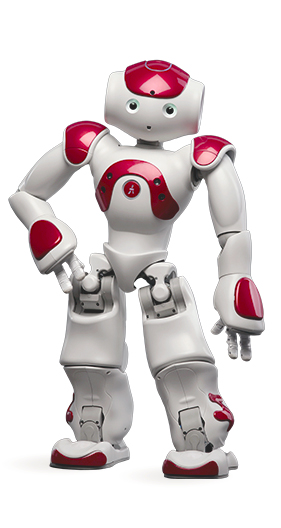
\includegraphics[scale=0.55]{images/nao-robot.jpg}\hfill
    \caption{NAO - Aldebaran Robotics \cite{aldebaran-masses}}\hfill
    \label{fig: nao-robot}
\end{figure}

NAO has a total of 25 degrees of freedom (DOF), 11 DOF for the lower part that includes legs and pelvis, and 14 DOF for the upper part that includes trunk, 
arms and head. Each leg has 2 DOF at the ankle, 1 DOF at the knee and 2 DOF at the hip. A special mechanism composed of two coupled joints at each hip equips 
the pelvis. The rotation axis of these two joints are inclined at $45^\circ$ towards the body. This mechanism replaces the classical set of three active rotary joints 
encountered in most humanoid robots.


Aldebaran Robotics provides a complete documentation for the robot, based on a geometric model shown in their website \cite{aldebaran-masses}. The model of the lower body of the robot 
NAO is obtained considering the two legs identical and identically actuated. The two revolute joints that constitute the pelvis and named separately, but 
they essentially represent a unique actuated DOF. To conclude, it is important to remark that, unlike prototypes such as Wabian-2R or LOLA, the foot sole of 
the present version of NAO does not feature any passive or active joint that would enhance higher speed gait performances.


\subsection{NAOqi C++ SDK}

The robot's embedded software, \textit{NAOqi}, a framework so the robot can be programmed in various operating systems, and in various languages, including C++, Python and MATLAB. 
The manufacturer also provides a software, \textit{choreographe} allows connecting to the real robot through local network and starts the NAOqi service in the robot.
\textit{Choreographe} can also be used as a graphical interface for block-programming to interact with the robot.

In this research, the software is developed in C++ for interaction with the real robot and compiled with CMake, a cross compiled platform for build systems, to make use of 
NAOqi libraries. The support for NAO v5 humanoid framework is provided in NAOqi version 2.1.4 and is used for both real robot and simulation. The NAOqi 2.1.4 applications could be build in unix-systems by custom cross-compiler \textit{qibuild}, a cmake extension and a python 2.7 module developed by Aldebaran 
Robotics. At the time of research, python 2.7 is completely abandoned. To make use of the functionalities of \textit{qibuild}, the module is built from source on python 3.8.

The software is developed on unix-system and ran in a seperate windows computer communicating with the robot through local network. The software is developed as a standalone build for suitable version control using \textit{git} and is available in 
\cite{github}.

\subsection{CopelliaSim support}
To simulate the dynamic behaviour during motion retargetting, the work is initially planned to simulate the robot in robotics simulators like Gazebo, Webots and CopelliaSim. 
The support for Webots and Gazebo has been dropped by Aldebaran community at the time of the research. Hence, the existing model of NAO robot in CopelliaSim is used to interact 
with NAOqi services and proxies. 


\begin{figure}[h!]
    \centering
    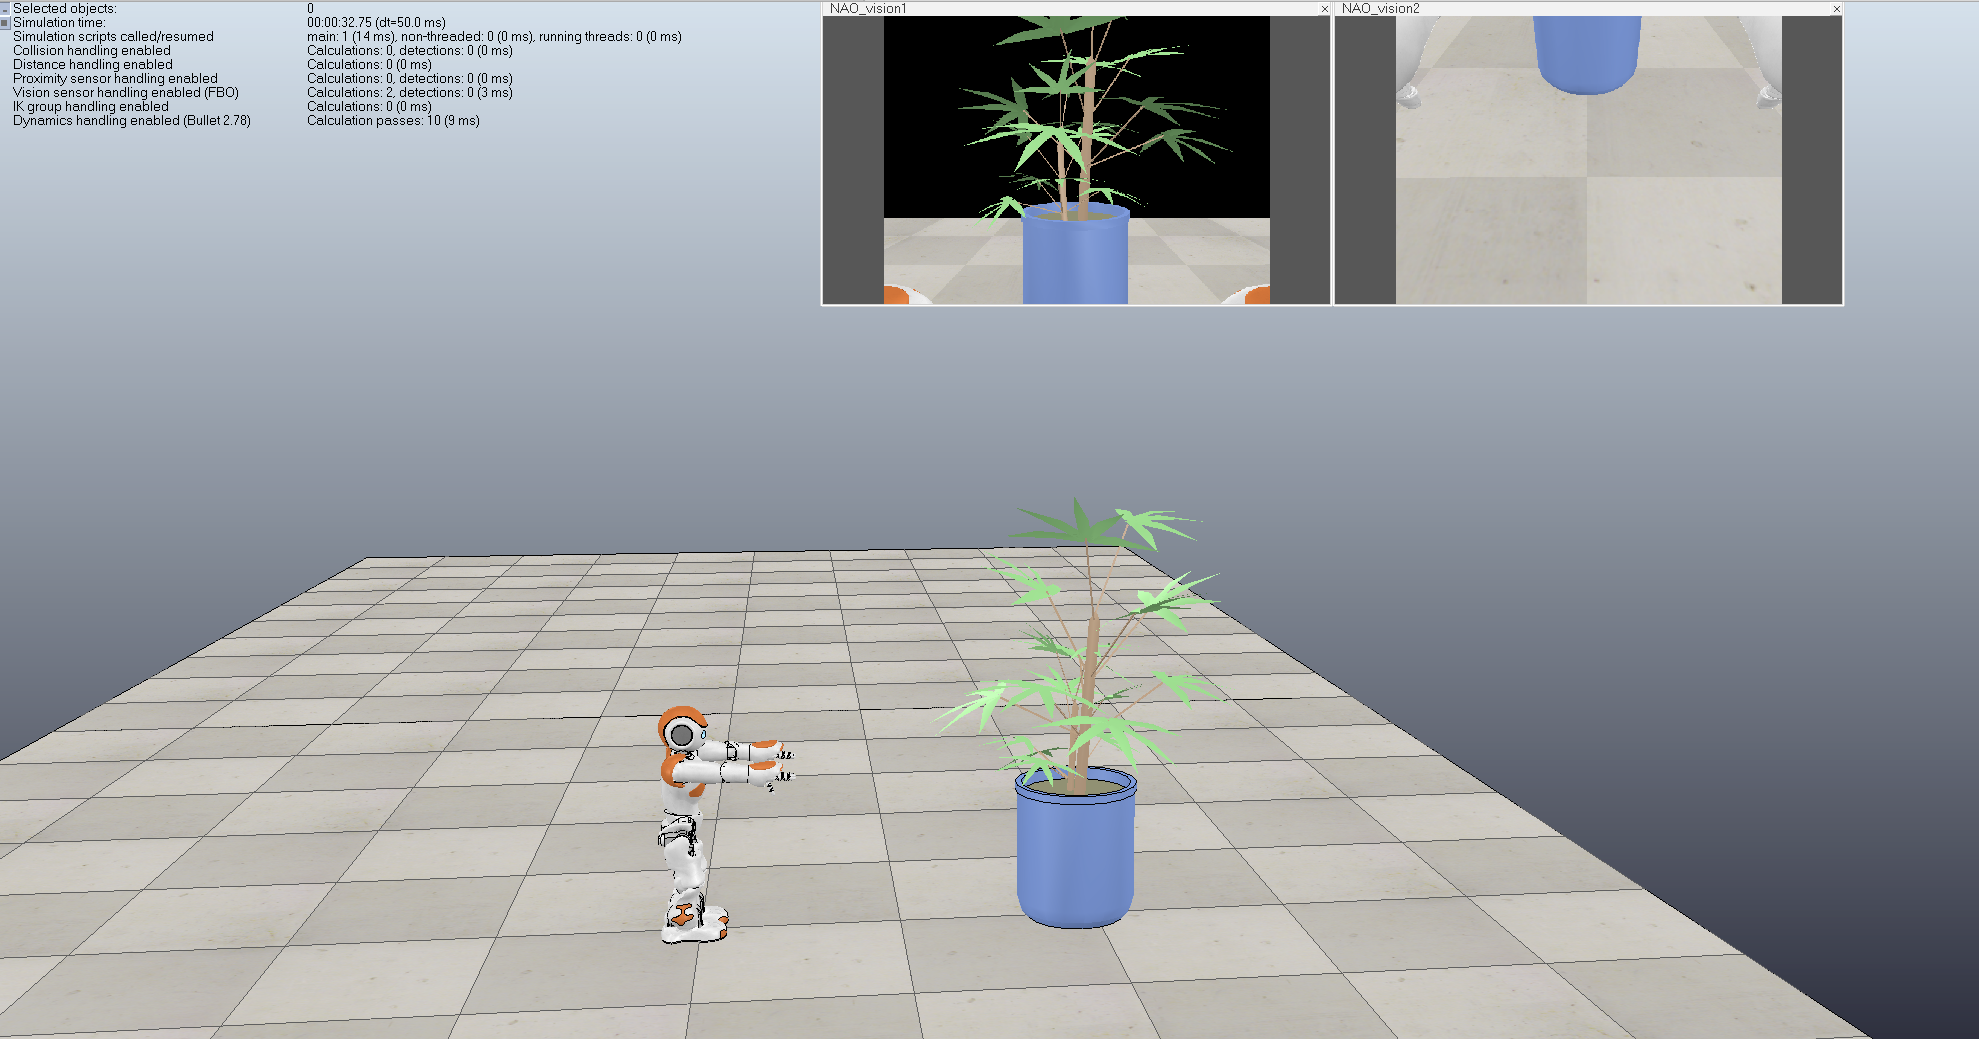
\includegraphics[scale=0.235]{images/copellia-sim.png}\hfill
    \caption{NAO robot in CopelliaSim simulator}\hfill
    \label{fig: copellia-sim}
\end{figure}

Figure \ref{fig: copellia-sim} presents the simulation of NAO robot and the interaction of Visual proxies from NAOqi services. The simulation is 
used as a testing platform to monitor the initial behaviour during the imitation process, although there are evidences that the simulators doesn't replicate exactly the dynamic 
behaviour of the humanoid robot in the real world \cite{ramosponce}. 

\section{Xsens MVN Analyze}


\subsection{Sensor Setup}
\subsection{Xsens Networking Protocol}
\subsection{Network Streaming}

\begin{figure}[h!]
    \centering
    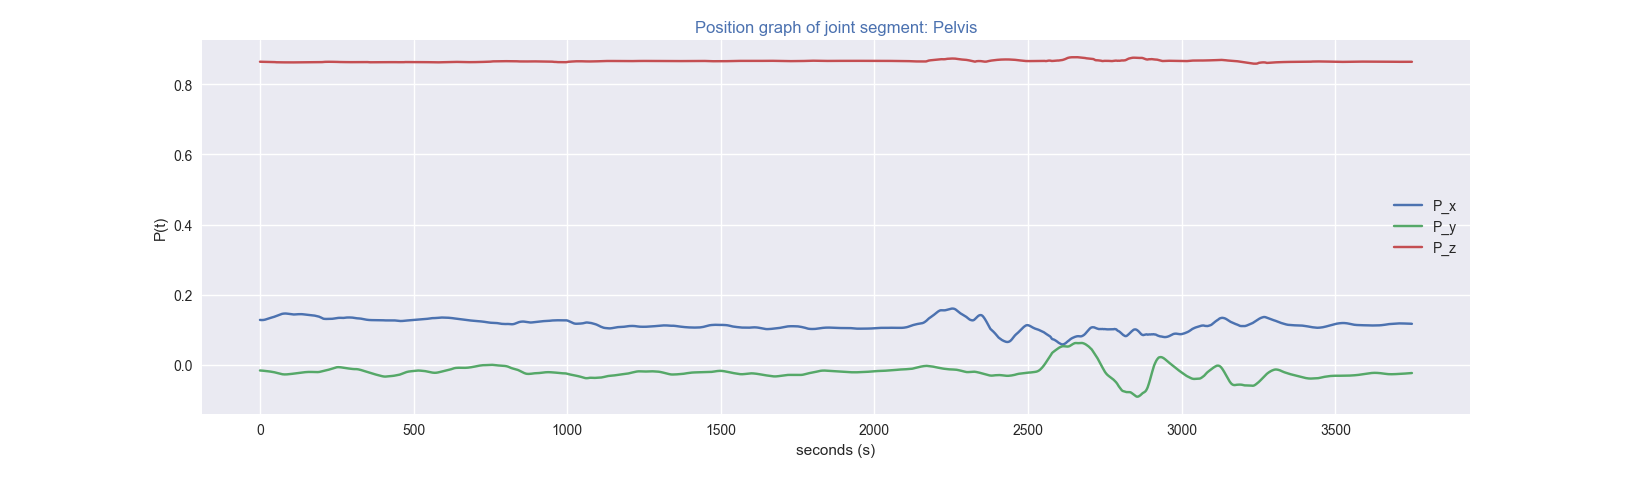
\includegraphics[scale=0.435]{images/xsens-pelvis-position.png}\hfill
    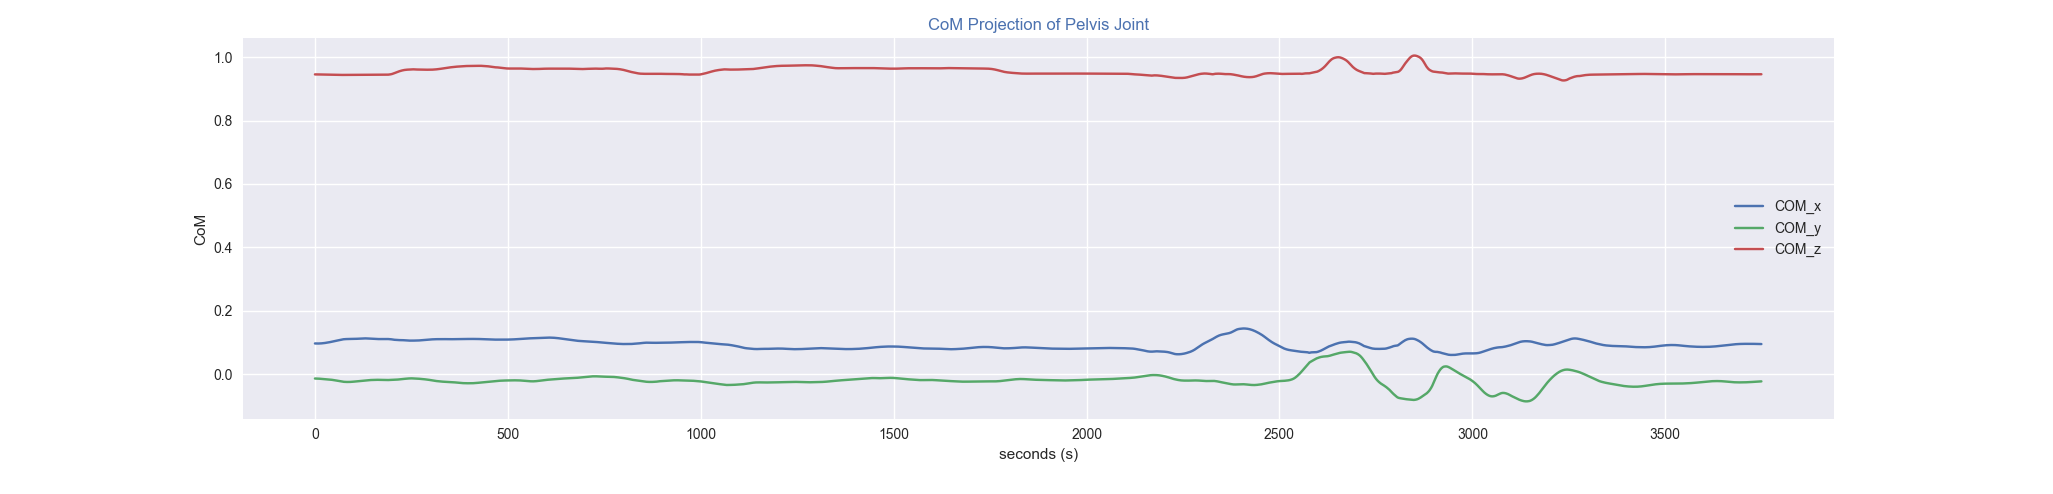
\includegraphics[scale=0.35]{images/xsens-pelvis-com.png}\hfill
    \caption{Xsens data plot pelvis joint}\hfill
    \label{fig: xsens-plot}
\end{figure}